%
%     巻頭言
%

\documentclass[10pt,b5paper,papersize,dvipdfmx]{jsbook}

\usepackage{vuccaken}
\usepackage{vuccaken2019}

% --------------------------------------
\begin{document}

\begin{preface}{巻頭言}
        {会長}% position
        {機械工学科2回生}% belong
        {\vname{西條}{晴幸}}% name
        {令和元年11月29日}% date
  %%
  物理科学研究会会長の西條晴幸です。今年度は令和最初の年であり、時代が節目を迎える年ですね。
  そんな中、我が物理科学研究会も二つの意味で節目を迎えていました。
  ひとつは弊研究会の全身である核物理研究会の1949年発足から数えて70周年を迎えること、もうひとつはここ2年間で新入会員が1人のみといういよいよ廃部の危機的な意味で、です。
  今年会員が入らなければ本当にいや、危なかった...
  ここで登場するのが敏腕新歓担当さいj嘘ですひとえに前会長、前々会長による物理科学科新入生への積極的な働きかけにより、約5人もの新入会員を迎え入れることができました。
  歴史的に見てもここ数年で70周年を迎える学友会諸団体は多く、それらと肩を並べてここまで弊研究会が続いて来られたのは先輩方の途切れることのない活動のためです。
  この70というひとつの節目を、これからの存続を感じさせる状態(会員獲得)で迎えられたことは非常に喜ばしいと感じています。\par
  さてこの会誌の内容ですが、これは主に弊研究会の半期の活動の結集となっています。会員それぞれが自分の興味ある分野について研究し、それを発表しあうというのが普段の活動ですが、それを形あるものにまとめたのがこの会誌という集大成なのです。分野については物理だけでなく、数学や多様な応用科学も対象としています。量子力学を完全に理解すると意気込んでいる人から論理学について書いた人まで様々です。\par
  そんなわけで会員増加に伴い、今回の会誌は中々多様な内容を詰め込んだものになっています。あなたの関心を引くものもきっとあることでしょう。あってほしい(願望)。章ごとに繋がりはなく、それぞれ読み切りなので軽い気持ちで好きなところだけでも読んでいっていただけると幸いです。それではどうぞ。\par
  年一の新刊を落としてしまった会長と1回生約1名は落とし前のつけ方についてでも考えておきます。
\end{preface}


%%
\clearpage
\quad\vfill
\begin{figure}[htb]
  \centering
  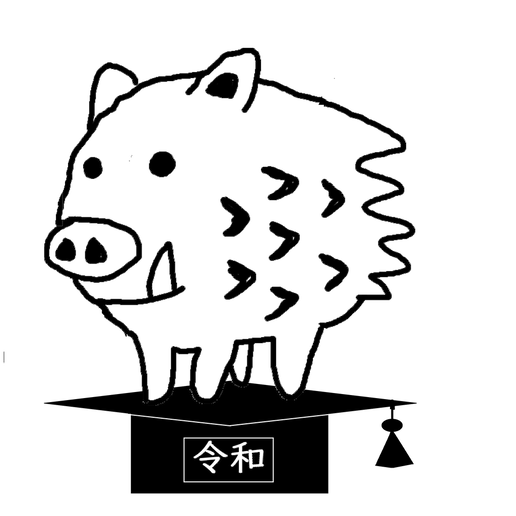
\includegraphics[width=40mm]{img/inoshishi.png}
  \caption*{
    \setlength{\baselineskip}{1.2zw}\gtfamily
    ボツ表紙 \\ 作・西村宗悟
  }
  \label{}
\end{figure}
\vfill

\end{document}
%
% お疲れさまです
%